 
\textbf{Instrucciones:} Cuenta con $1$ y $30$ minutos para la realización de este control. No está permitido el uso de calculadora.
 
\vspace{0.5cm}
\setlength\parindent{0pt} \textbf{\large Pregunta 1} \\
\textbf{Esta pregunta está compuesta de 3 partes independientes.}\\
\textbf{Parte 1}:
Considere el sistema electromecánico presentado en Figura \ref{fig:1}. El objetivo del sistema es controlar la
posición de la bola ajustando la corriente en el electroimán mediante el voltaje
de entrada $e(t)$. Notar que la fuerza magnética que interactúa con la bola de acero queda descrita por $i^2/y$. 
\begin{figure}
    \centering
    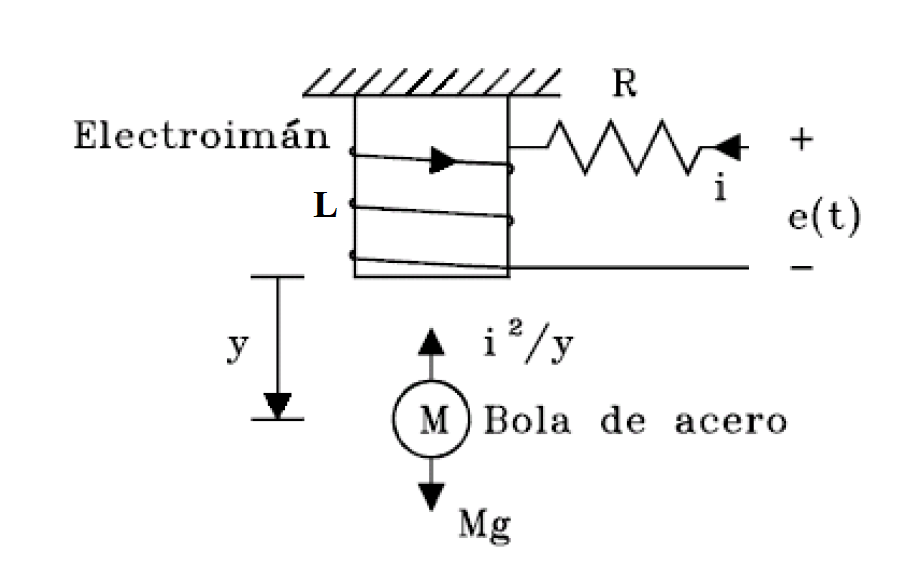
\includegraphics[width=0.6\linewidth]{img/C1_figura.png}
    \caption{Modelo simplificado de levitación magnética.}
    \label{fig:1}
\end{figure}

Las ecuaciones que describen el comportamiento del sistema se pueden obtener aplicando la segunda ley de Newton a la bola y la ley de Kirchhoff al circuito eléctrico:

